\hypertarget{_sample_stream_8cpp}{}\section{Visual\+Impro/\+Sample\+Stream.cpp File Reference}
\label{_sample_stream_8cpp}\index{Visual\+Impro/\+Sample\+Stream.\+cpp@{Visual\+Impro/\+Sample\+Stream.\+cpp}}


Object used to contain a wavefile.  


{\ttfamily \#include $<$Sample\+Stream.\+hpp$>$}\newline
Include dependency graph for Sample\+Stream.\+cpp\+:
\nopagebreak
\begin{figure}[H]
\begin{center}
\leavevmode
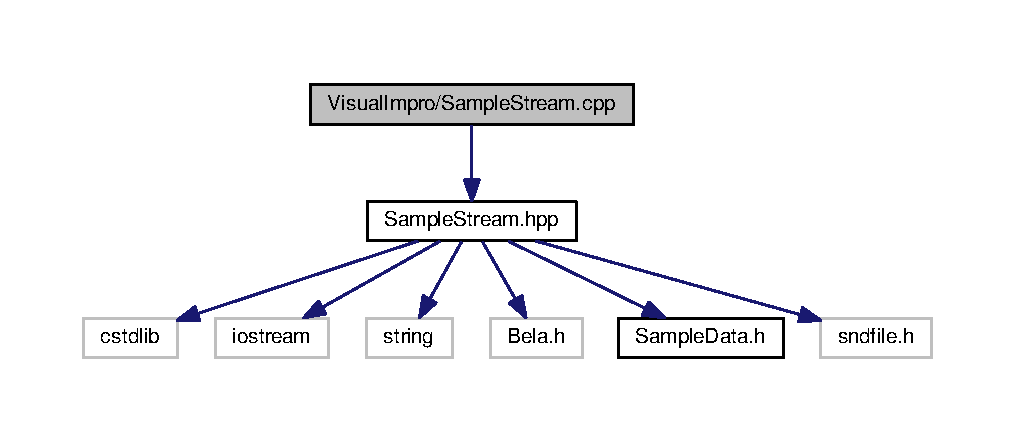
\includegraphics[width=350pt]{_sample_stream_8cpp__incl}
\end{center}
\end{figure}


\subsection{Detailed Description}
Object used to contain a wavefile. 

\begin{DoxyAuthor}{Author}
Jérémy L\+I\+X\+A\+N\+D\+RE 
\end{DoxyAuthor}
\begin{DoxyDate}{Date}
July 2017
\end{DoxyDate}
The \mbox{\hyperlink{class_sample_stream}{Sample\+Stream}} object is here to contain wavefiles for out program and used in render.\+cpp. It is represented in our program as an orray of \mbox{\hyperlink{class_sample_stream}{Sample\+Stream}} objects for representing all of our wavefiles only. 